\chapter{Introduction}

% let's show you how \cite and \gls for abbreviations works
Example paragraph: 

Niemann~\cite{Niemann83KVM} wrote a nice book. There is no \glspl{svm} defined,
but maybe he said something about Bayesian classifiers, maybe here~\cite[p.34]{Niemann83KVM}.
But I like \glspl{svm}, so give me an \gls{svm}. 

Useful reads:

Checkout the subcaption package how to do multiple figures/tables. Make sure
that you use vector graphics - no blurry png - for graphs or similar, \eg use
tikz/inkscape. \cref{fig:ex} is an example of a figure using the package tikz. Make also sure that your plots are readable and have axis
captions, \eg use pgfplots.

How to create good looking tables with the booktabs package
e.g. a table should like \cref{tab:ex}.

\begin{table}
    \centering
        \caption[Short title for the List of Tables.]{Long caption for this table which is composed by sub-table 1 and sub-table 2.}
        \begin{subtable}{.5\textwidth}
            \centering
                \caption{Sub-table 1.}
            	\begin{tabular}{llr}
            		\toprule
            		id & method & result\\
            		\midrule
            		1 & A & 0.9\\
            		2 & B & 0.8\\
            		\bottomrule
            	\end{tabular}
        \end{subtable}% <---- don't forget this %
        \begin{subtable}{.5\textwidth}
            \centering
                \caption{Sub-table 2.}
            	\begin{tabular}{llr}
            		\toprule
            		id & method & result\\
            		\midrule
            		1 & C & 90\%\\
            		2 & D & 80\%\\
            		\bottomrule
            	\end{tabular}
        \end{subtable}
\label{tab:ex}
\end{table}


\begin{figure}
\centering
 \centering
 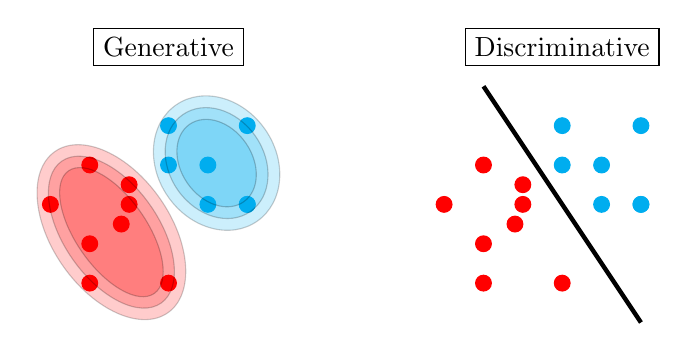
\begin{tikzpicture}[scale=0.5]
  \node[draw] at (3,7) {Generative};

  \draw[draw=red,fill=red] (1,1) circle (0.2);
  \draw[draw=red,fill=red] ( 2 , 3.5 ) circle (0.2);
  \draw[draw=red,fill=red] ( 0 , 3 ) circle (0.2);
  \draw[draw=red,fill=red] ( 1 , 2 ) circle (0.2);
  \draw[draw=red,fill=red] ( 2 , 3 ) circle (0.2);
  \draw[draw=red,fill=red] ( 3 , 1 ) circle (0.2);
  \draw[draw=red,fill=red] ( 1 , 4 ) circle (0.2);
  \draw[draw=red,fill=red] (1.8,2.5) circle (0.2);
  %
  \draw[rotate around={35:(2,2)},fill=red, opacity=0.2] (1.8,2.5) ellipse (1.5 and 2.5);
  \draw[rotate around={35:(2,2)},fill=red, opacity=0.21] (1.8,2.5) ellipse (1.2 and 2.2);
  \draw[rotate around={35:(2,2)},fill=red, opacity=0.22] (1.8,2.5) ellipse (0.9 and 1.9);
  %%%%%%%%%%%%%%%%%%%%%
  \draw[draw=cyan,fill=cyan] ( 4 , 3 ) circle (0.2);
  \draw[draw=cyan,fill=cyan] ( 4 , 4 ) circle (0.2);
  \draw[draw=cyan,fill=cyan] ( 5 , 5 ) circle (0.2);
  \draw[draw=cyan,fill=cyan] ( 5 , 3 ) circle (0.2);
  \draw[draw=cyan,fill=cyan] ( 3 , 4 ) circle (0.2);
  \draw[draw=cyan,fill=cyan] ( 3 , 5 ) circle (0.2);
  \draw[draw=cyan,fill=cyan] ( 5 , 3 ) circle (0.2);
  \draw[rotate around={35:(4.5,4)},fill=cyan, opacity=0.2] (4.3,4.2) ellipse (1.5 and 1.8);
  \draw[rotate around={35:(4.5,4)},fill=cyan, opacity=0.21] (4.3,4.2) ellipse (1.2 and 1.5);
  \draw[rotate around={35:(4.5,4)},fill=cyan, opacity=0.22] (4.3,4.2) ellipse (0.9 and 1.2);
  %%%%%%%%%%%%%%%%%%%%%%%%%%%%%%%%%%%%%%%%%
  \node[draw] at (13,7) {Discriminative};
  \draw[ultra thick] (15,0) -- (11,6cm);
  \draw[draw=red,fill=red] ( 11 , 1 ) circle (0.2);
  \draw[draw=red,fill=red] ( 12, 3.5) circle (0.2);
  \draw[draw=red,fill=red] ( 10 , 3 ) circle (0.2);
  \draw[draw=red,fill=red] ( 11 , 2 ) circle (0.2);
  \draw[draw=red,fill=red] ( 12 , 3 ) circle (0.2);
  \draw[draw=red,fill=red] ( 13 , 1 ) circle (0.2);
  \draw[draw=red,fill=red] ( 11 , 4 ) circle (0.2);
  \draw[draw=red,fill=red] (11.8,2.5) circle (0.2);
  %%%%%%%%%%%%%%%%%%%%%
  \draw[draw=cyan,fill=cyan] ( 14 , 3 ) circle (0.2);
  \draw[draw=cyan,fill=cyan] ( 14 , 4 ) circle (0.2);
  \draw[draw=cyan,fill=cyan] ( 15 , 5 ) circle (0.2);
  \draw[draw=cyan,fill=cyan] ( 15 , 3 ) circle (0.2);
  \draw[draw=cyan,fill=cyan] ( 13 , 4 ) circle (0.2);
  \draw[draw=cyan,fill=cyan] ( 13 , 5 ) circle (0.2);
  \draw[draw=cyan,fill=cyan] ( 15 , 3 ) circle (0.2);
 \end{tikzpicture}
\caption{Example of a figure using the package \textit{tikz}}
\label{fig:ex}
\end{figure}
